\documentclass{beamer}
\usetheme{Warsaw}
\setbeamertemplate{footline}[frame number]

\usefonttheme[]{serif}
\usepackage{amsmath, latexsym, color, graphicx}
\usepackage{epsf, epsfig}
\usepackage{amsfonts,multicol}

\newcommand{\tbs}{\textbackslash}
\definecolor{cRed}{rgb}{1, 0, 0}

\title{\LaTeX{} Gotchas - Common Pitfalls and Debugging}
\author{Christopher Rose}
\institute{Electrical and Computer Engineering \\ Auburn University}
\date{\today}

\begin{document}
%%%%%%%%%%%%%%%%%%%%%%
%Frame 
\maketitle

\section{Introduction}

%%%%%%%%%%%%%%%%%%%%%%
%Frame 
\begin{frame}
\frametitle{Outline}
\tableofcontents[currentselection]
\end{frame}

%%%%%%%%%%%%%%%%%%%%%%
%Frame 
\begin{frame}
\frametitle{Introduction}

\LaTeX
\begin{itemize}
\item is easy
\item has a steep learning curve
\end{itemize}
With enough experience, errors are recognized and easily fixed.

\end{frame}

\section{Installation and Setup}
\subsection{TeXnicCenter Installation}
%%%%%%%%%%%%%%%%%%%%%%
%Frame 
\begin{frame}[fragile]
\frametitle{TeXnicCenter Installation}
\begin{block}{Compatibility Error}
\begin{verbatim}
GUI framework cannot be initialized
\end{verbatim}
\end{block}

\begin{itemize}
\item occurs when a missing package must be installed and the pop up message cannot be displayed
\item fix: allow package installations to occur automatically
\end{itemize}
\end{frame}

%%%%%%%%%%%%%%%%%%%
%Frame
\begin{frame}
\frametitle{TeXnicCenter Installation}
\begin{figure}[htbp]
\centering
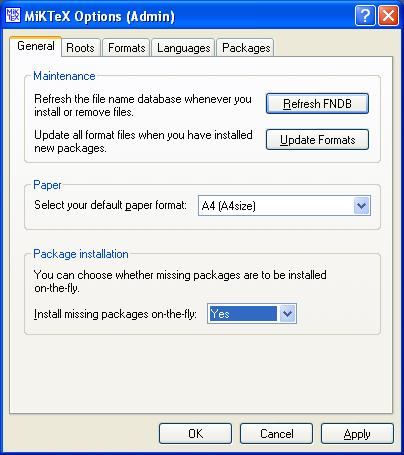
\includegraphics[width=5cm]{NotOnFly.jpg}
\caption{TeXnicCenter Compatibility Fix}
\label{fig::compatFix}
\end{figure}
\end{frame}


%%%%%%%%%%%%%%%%%%%%%%
%Frame 
\begin{frame}
\frametitle{TeXnicCenter Installation}
\begin{figure}[htbp]
\centering
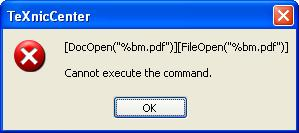
\includegraphics[width=5cm]{openIssue.jpg}
\caption{Output Display Failure}
\label{fig::openIssue}
\end{figure}

Often while using pdflatex you will see the above pop up displayed.  This can happen for several reasons:

\begin{itemize}
\item Build failed - pdf file was not created
\item Output profile incorrectly setup
\item need to close TeXnicCenter
\end{itemize}

\end{frame}

%%%%%%%%%%%%%%%%%%%%%%
%Frame 
\begin{frame}
\frametitle{TeXnicCenter Installation}
The installation asks for the path to your .pdf reader and .dvi reader.  If you do not specify a path, you will have to manually go to the folder and open the created .pdf file.  If you do not close the file and try building and viewing your file, you will get the following error:

\begin{figure}[htbp]
\centering
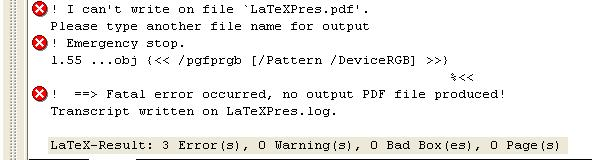
\includegraphics[width=8cm]{Icantwrite.jpg}
\caption{Unable to write on file}
\label{fig::Icantwrite}
\end{figure}
\end{frame}

\subsection{TeXnicCenter Output Profiles}

%%%%%%%%%%%%%%%%%%%%%
%Frame
\begin{frame}
\frametitle{TeXnicCenter Output Profiles}
\setbeamercovered{invisible}

The solution is defining your viewer in the output profile:

\only<1>{
\begin{figure}[htbp]
\centering
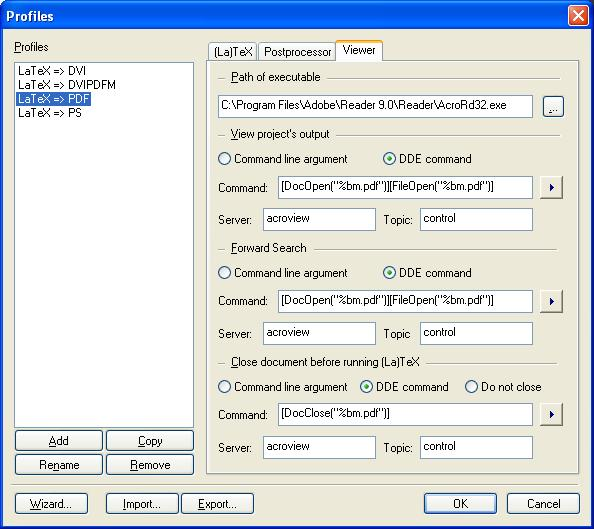
\includegraphics[width=6cm]{outputProfileViewer.jpg}
\caption{Output Profile - Viewer Tab}
\label{fig::outputProfileViewer}
\end{figure}
}
\only<2>{
\begin{figure}[htbp]
\centering
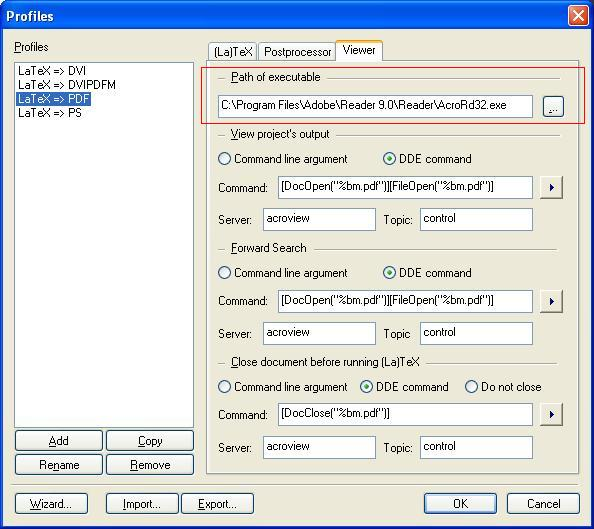
\includegraphics[width=6cm]{outputProfileViewer2.jpg}
\caption{Output Profile - Viewer Tab}
\label{fig::outputProfileViewer2}
\end{figure}
}

\only<3>{
\begin{figure}[htbp]
\centering
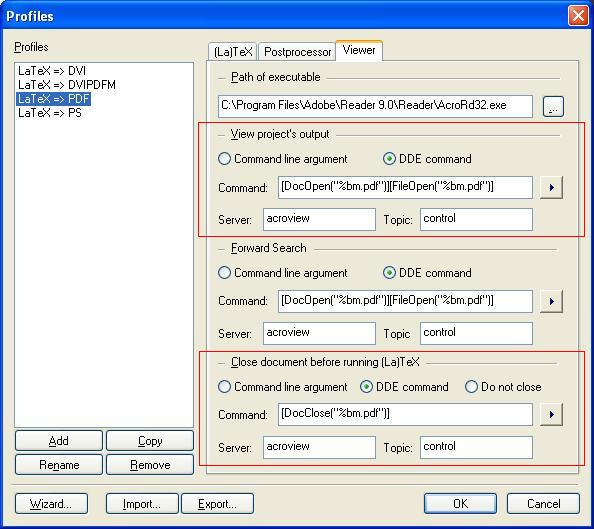
\includegraphics[width=6cm]{outputProfileViewer3.jpg}
\caption{Output Profile - Viewer Tab}
\label{fig::outputProfileViewer3}
\end{figure}
}

\end{frame}

\begin{frame}
\frametitle{TeXnicCenter Output Profiles}
The path of executable for your viewer, if wrong or nonexistent, results in:

\begin{itemize}
\item the output failing to be shown
\item failure to close the currently opened document
\end{itemize}

If the path to your executable changes, such as a new version of Adobe Acrobat, the path to the executable must be updated.

\end{frame}

\begin{frame}
\frametitle{Spelling}
``Check spelling while typing'' can be turned on in the Tools$\rightarrow$ Options menu in TeXnicCenter.

\begin{columns}
\column{.4\textwidth}

\begin{figure}[htbp]
\centering
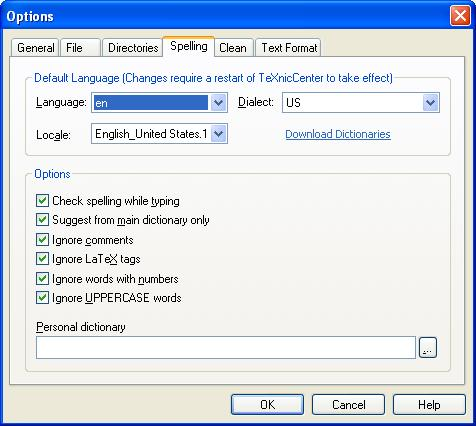
\includegraphics[width=4cm]{spelling.jpg}
\caption{Check Spelling}
\label{fig::spelling}
\end{figure}

\column{.4\textwidth}

\begin{figure}[htbp]
\centering
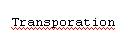
\includegraphics[width=3cm]{misspelled.jpg}
\caption{Misspelled}
\label{fig::misspelled}
\end{figure}

\end{columns}

\end{frame}

\section{Common Errors}
\subsection{Error Messages}
%%%%%%%%%%%%%%%%%%%%%%
%Frame 
\begin{frame}[fragile]
\frametitle{Error Format}

\begin{block}{Example Error Message}

\begin{verbatim}
! Undefined control sequence.
1.6 \tableofcotnetns
\end{verbatim}

\end{block}

Error messages begin with an exclamation mark and a description of the error.  On the second line is the line number in the document that \LaTeX \ was processing at the time.  This error is showing that \begin{verbatim}\tableofcontents \end{verbatim} is misspelled.

\end{frame}

\begin{frame}[fragile]
\frametitle{Error Messages}
\begin{block}{Example Error Messages}

\begin{verbatim}
! Too many }'s.
1.6 \date December 2004}
\end{verbatim}

\end{block}

Too many curly braces often means a problem in an equation.  Here the open curly brace was left out after the \begin{verbatim}\date{}\end{verbatim} command.

\end{frame}

\begin{frame}[fragile]
\frametitle{Error Messages}

\begin{block}{Example Error Message}
\begin{verbatim}
! LaTeX Error: File `aums.sty' not found.
Type X to quit or <RETURN> to proceed,
or enter new name.
\end{verbatim}
\end{block}

This error arises when the \LaTeX \ style file cannot be found.

\end{frame}

\begin{frame}[fragile]
\frametitle{Error Messages}

\begin{block}{Example Error Message}
\begin{verbatim}
Runaway argument?
{December 2004 \maketitle
! Paragraph ended before \date was complete.
<to be read again>
\par
l.8
\end{verbatim}
\end{block}

This error arises from not closing the curly brace.  \LaTeX \ is still expecting more text for the date while trying to format the entire title page.  The error is detected as $\backslash$maketitle creates new paragraphs, and the error is thrown.

\end{frame}

\subsection{Warning Messages}

\begin{frame}[fragile]
\frametitle{Warning Messages}

\begin{block}{Example Warning Message}
\begin{verbatim}
Underfull \hbox (badness 1394) in paragraph
at lines 28--30
[][]\LY1/brm/b/n/10 Bull, RJ: \LY1/brm/m/n/10
En-gine--ering in-
[102]
\end{verbatim}
\end{block}

This warning shows that \LaTeX \ cannot stretch the line wide enough to fit the line without making the spacing bigger than is maximally currently permitted.  The badness (0-10000) indicates its severity.  The codes separated by slashes are the typeface, font style, and size used in the line.  The number in brackets is the page number.

\end{frame}

\begin{frame}[fragile]
\frametitle{Warning Messages}

\begin{block}{Example Warning Message}
\begin{verbatim}
[101]
Overfull \hbox (9.11617pt too wide) in paragraph
at lines 670--671
[]\LY1/brm/b/n/10 Windows, \LY1/brm/m/it/10 see
\LY1/brm/m/n/10 X Win-
\end{verbatim}
\end{block}

This warning shows that the line is too wide to fit on the line.  The chosen hyphenation point that minimizes the error is shown at the end (Win-).  If the overfull word includes a forward slash, the slash should be written using $\backslash$slash since it can be broken across lines.

\end{frame}

\begin{frame}
\frametitle{Common Errors}
Word documents are single files.

\LaTeX \ documents have many files associated with them.

\begin{figure}[htbp]
\centering
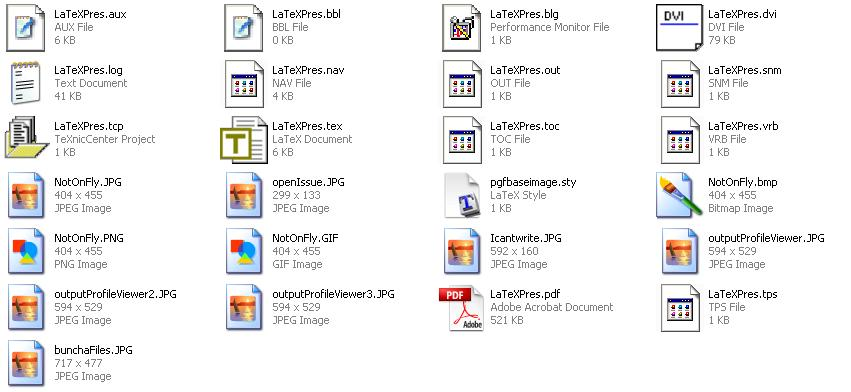
\includegraphics[width=7cm]{bunchaFiles.jpg}
\caption{Files in Working Directory}
\label{fig::bunchaFiles}
\end{figure}
Each \LaTeX \ document should have its own folder.

\end{frame}

\subsection{Special Characters}

%%%%%%%%%%%%%%%%%%%%%%
%Frame 
\begin{frame}[fragile]
\frametitle{Common Errors}

\begin{itemize}

\item Special Characters
\begin{itemize}
\item \%
\item \$
\item \{ \ \}
\item /
\item $\backslash$ : spaces after special characters
\end{itemize}

\item hyperref package must be listed last
\item Math Mode
\item Preamble errors

\end{itemize}

\end{frame}

\begin{frame}[fragile]
\frametitle{Copy \& Paste}

Much of working with LaTeX involves copy and pasting previous \LaTeX \ code, such as for figures, arrays, and tables.  Copy and pasting incorrect sections of code can cause errors.

\begin{block}{Example}
\begin{verbatim}
\begin{figure}[htbp]
\centering
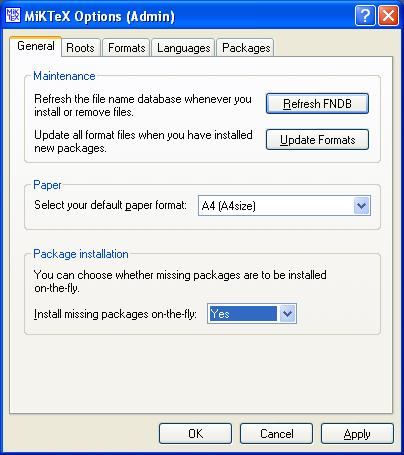
\includegraphics[width=5cm]{NotOnFly.jpg}
\caption{TeXnicCenter Compatibility Fix}
\label{fig::compatFix}
\end{figure}
\end{figure}
\end{verbatim}
\end{block}

\end{frame}

\section{Figures}
\subsection{Graphic Options}
%%%%%%%%%%%%%%%%%%%%%%
%Frame 
\begin{frame}
\frametitle{Figures - Graphic Options}
Two options are available for graphics
\begin{itemize}
\item include PostScript(.eps,.ps) images
\item include PDF, PNG, and JPEG images
\end{itemize}

Mixing the incompatible image formats will result in errors.

An option is available for converting .dvi to .pdf called dvipdfm which converts a .dvi file directly into .pdf.  Alternatively, you can convert the .dvi file to a .ps file which can then be converted to a .pdf.

\end{frame}

\begin{frame}
\frametitle{Figures - Graphic Options}
\begin{figure}[htbp]
\centering
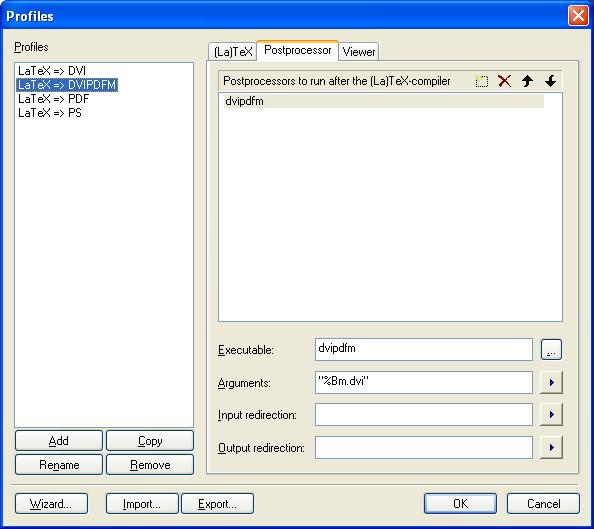
\includegraphics[width=5cm]{dvipdfm.jpg}
\caption{Setup for dvipdfm in Profiles of TeXnicCenter}
\label{fig::dvipdfm}
\end{figure}
\end{frame}

\subsection{Bad Boxes}

\begin{frame}
\frametitle{Figures - Bad Boxes}
Bad box warning in the \LaTeX{} result is normally due to graphics extending past the limits of the page.  It may also be due to failure of \LaTeX \ to justify text, and the text edges out over the margin.

\begin{figure}[htbp]
\centering
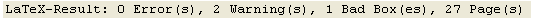
\includegraphics[width=9cm]{badboxwarning.png}
\caption{Bad Box warning}
\label{fig::badboxwarning}
\end{figure}

\begin{figure}[htbp]
\centering
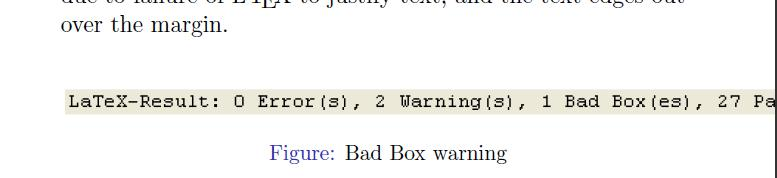
\includegraphics[width=6cm]{overflow.jpg}
\caption{Example of Figure going outside of the frame}
\label{fig::overflow}
\end{figure}
\end{frame}

\subsection{Placement}

\begin{frame}
\frametitle{Figures - Placement}
\LaTeX{} places floats automatically in order to make it look as nice as possible.  If not enough room is present, then the figure will be moved to the next page, and the text following the figure in your .tex document will take its place.\\
\vspace{1cm}
This can be a problem if your professor wants the document a specific way and is used to Word.
  
\end{frame}

\begin{frame}
\frametitle{Figures - Placement}
Another problem that may come up is if the figure does not fit the body well and is pushed to the end of the section.  Since the figures must appear in order, all following figures will go with it.  \\
\vspace{1cm}
Result: Text $\rightarrow$ figures
\end{frame}

\begin{frame}
\frametitle{Links}
http://en.wikibooks.org/wiki/LaTeX/ \\
http://www.tug.org/TUGboat/Articles/tb26-1/schwartz.pdf\\

\end{frame}

\section{Conclusion}
%%%%%%%%%%%%%%%%%%%%%%
%Frame 
\begin{frame}
\begin{center}
\frametitle{Conclusions}
\Huge Google it!\\
\tiny or use the search engine of your choice\\
\vspace{1cm}
\huge Questions?
\end{center}
\end{frame}

\end{document}